\begin{center}
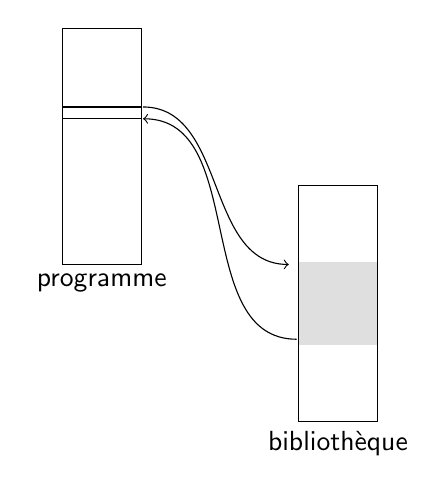
\begin{tikzpicture}
  \draw (0,2) rectangle (1,5);

  \draw (3,0) rectangle (4,3);
    

  \node (a) at (0.9, 4) {};
  \node (b) at (3, 2) {};
  \node (c) at (3.1, 1.05) {};
  \node (d) at (0.9, 3.85) {};
  \draw[->] (a)  to [out=0,in=180] (b);
  \draw[->] (c)  to [out=180,in=0] (d);

  \draw (3.5,0) node [below] {\textsf{bibliothèque}};
  \draw (0.5,2.) node [below] {\textsf{programme}};

  \fill[gray,opacity=0.25] (3, 0.975) rectangle (4,2.025);
  \draw (0,4) -- (1,4);
  \draw (0,3.85 ) -- (1,3.85);
\end{tikzpicture}
\end{center}
